\documentclass{article}
% Elsevier graphical-abstract proportion, 1328 x 531 px (w x h)
\usepackage[paperwidth=26.56cm,paperheight=10.62cm,margin=4mm]{geometry}
\usepackage[T1]{fontenc}
\usepackage{stix}
\usepackage{tikz}
\usetikzlibrary{arrows.meta,calc,positioning}
\pagestyle{empty}
\newcommand{\COtwo}{CO\textsubscript{2}}
\begin{document}
\centering
{\LARGE\bfseries Shared ePC-SAFT water, \COtwo{} and inorganic-ion parameters for \COtwo-loaded aqueous amines}\par
\vspace{1.5mm}
{\large Equilibrium constants fixed at literature correlations, except carbamate hydrolysis of DEA and AMP, which is fitted}\par
\vspace{9mm}
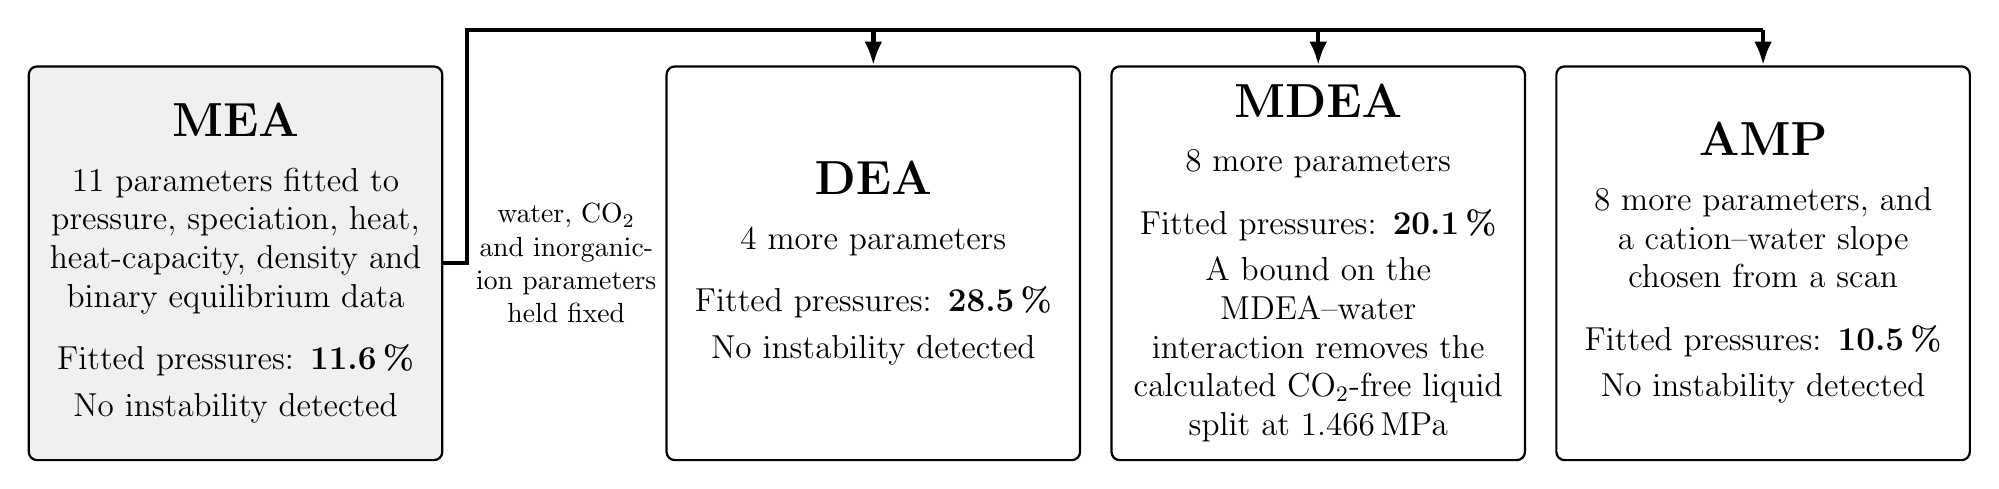
\begin{tikzpicture}[box/.style={draw, rounded corners=3pt, line width=0.8pt, align=center, text width=4.9cm, minimum height=5.0cm, inner sep=5pt, anchor=north west, font=\large}]
\node[box, fill=gray!12] (mea) at (0,0) {{\LARGE\bfseries MEA}\\[2mm] 11 parameters fitted to\\ pressure, speciation, heat,\\ heat-capacity, density and\\ binary equilibrium data\\[3mm] Fitted pressures: \textbf{11.6\,\%}\\[1mm] No instability detected};
\node[box] (dea) at (8.1,0) {{\LARGE\bfseries DEA}\\[2mm] 4 more parameters\\[3mm] Fitted pressures: \textbf{28.5\,\%}\\[1mm] No instability detected};
\node[box] (mdea) at (13.75,0) {{\LARGE\bfseries MDEA}\\[2mm] 8 more parameters\\[3mm] Fitted pressures: \textbf{20.1\,\%}\\[1mm] A bound on the MDEA--water\\ interaction removes the\\ calculated CO$_2$-free liquid\\ split at 1.466\,MPa};
\node[box] (amp) at (19.4,0) {{\LARGE\bfseries AMP}\\[2mm] 8 more parameters, and\\ a cation--water slope\\ chosen from a scan\\[3mm] Fitted pressures: \textbf{10.5\,\%}\\[1mm] No instability detected};
% The shared parameters feed all three amines.
\coordinate (bus) at ($(mea.east)+(0.3,0)$);
\draw[line width=1.6pt] (mea.east) -- (bus) |- ($(amp.north)+(0,0.45)$);
\foreach \b in {dea, mdea, amp} \draw[-{Latex[length=3mm]}, line width=1.6pt] ($(\b.north)+(0,0.45)$) -- (\b.north);
\node[align=center, font=\normalsize] at ($(bus)!0.5!(dea.west)$) {water, CO$_2$\\ and inorganic-\\ion parameters\\ held fixed};
\end{tikzpicture}\par
\vspace{3mm}
{\large Fitted pressures: average absolute relative deviation of the fitted loaded-solution pressures. Splits from finite phase-stability searches.\\ The models are calibrations against data examined during development; they provide neither validation nor a basis for absorber design.}
\end{document}
